\section{Tecnologías utilizadas}\label{s:tech}
Antes de comenzar con el desarrollo del trabajo realizado, en esta sección se introducen las distintas tecnologías que han sido empleadas para la implementación del proyecto. Dado que el estudio gira en torno a los cuerpos de los correos electrónicos, es imprescindible un analizador sintáctico que facilite el estudio del corpus de partida. Para cubrir esta necesidad, se ha elegido spaCy, herramienta que se detalla en la sección \ref{ss:spacy}. Por otro lado, en lo relativo a las tareas relacionadas con el procesamiento de lenguaje natural, también se necesita poder obtener los Information Items dado un texto de entrada. Este problema puede implementarse gracias a la librería textaCy (véase el apartado \ref{ss:textacy}).

En cuanto al desarrollo de la arquitectura transformer, la cual consta de numerosas capas de redes neuronales, como se explicó en la sección \ref{sss:transformer}, será de gran ayuda la librería desarrollada por Google llamada Tensorflow (consúltese el apartado \ref{ss:tf}). Gracias a ella será posible presentar un modelo de aprendizaje automático que aborde todos los problemas de la generación de lenguaje natural.

Por último, se introduce el sistema de almacenamiento con el que se ha trabajado para contar con una gestión eficiente de los datos que se manejan: MongoDB (sección \ref{ss:mongodb}).

\subsection{spaCy}\label{ss:spacy}
Para ser capaces de llegar a conclusiones y estudiar el corpus de correos electrónicos seleccionado (véase la sección \ref{ss:enron}), se debe poder analizar el cuerpo de los mismos. Es decir, se necesita un analizador sintáctico que permita separar los diferentes textos en tokens (o dicho de otro modo, segmentar el texto en palabras, signos de puntuación, etcétera) y obtener diferentes características de ellos (como su categoría gramatical). Para conseguir ese objetivo, se va a utilizar la librería spaCy\footnote{\url{https://spacy.io/}}.

En esta sección se explican las razones por las que se elige spaCy (véase la sección \ref{ssect:spacywhy}) y su utilidad en el proyecto (véase la sección \ref{ssect:spacyut}).

\subsubsection{spaCy frente a otros analizadores sintácticos}\label{ssect:spacywhy}

Se ha elegido spaCy como analizador sintáctico frente a otros por varias razones, apoyadas por investigaciones publicadas como la realizada por \cite{choi2015depends}, y que se explican a continuación.

\begin{figure}[h]
	\centering%
	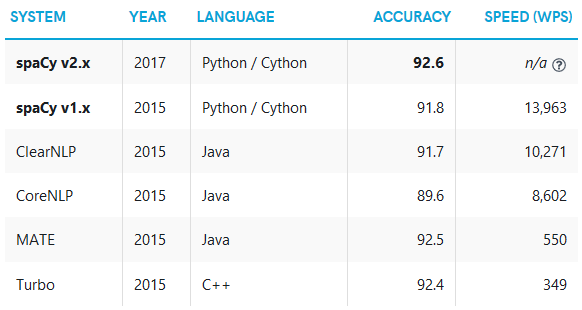
\includegraphics[width = 0.75\textwidth]{Imagenes/Bitmap/spacyeval.png}%
	\caption{Benchmarks de los distintos analizadores sintáctos}%
	Imagen extraída de \url{https://spacy.io/usage/facts-figures#benchmarks}
	\label{fig:spacyeval}
\end{figure}

Una evaluación publicada por \textit{Yahoo! Labs} y la Universidad Emory, como parte de un estudio de las tecnologías de análisis sintáctico actuales \citep{choi2015depends}, observó que ``spaCy es el analizador sintáctico voraz más rápido'' y su precisión está dentro del 1\% de los mejores existentes (como podemos ver en la figura \ref{fig:spacyeval}). Los pocos sistemas que son más precisos son, al menos, 20 veces más lentos. La velocidad es un factor importante cuando se quiere implementar sistemas complejos que se enfrentan a textos largos o a un gran número de documentos (como es el caso de este trabajo, en el que se quieren analizar todos los correos electrónicos posibles).

\begin{figure}[h]
	\centering%
	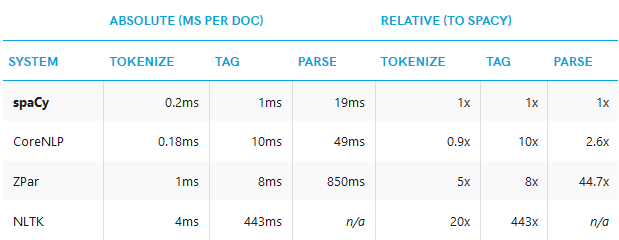
\includegraphics[width = 0.85\textwidth]{Imagenes/Bitmap/spacyspeed.png}%
	\caption{Tiempo de procesamiento por documento de varias librerías de NLP}%
	Imagen extraída de \url{https://spacy.io/usage/facts-figures#benchmarks}
	\label{fig:spacyspeed}
\end{figure}

Los resultados de \cite{choi2015depends} y las discusiones posteriores ayudaron a spaCy a desarrollar una novedosa técnica para mejorar la precisión del sistema, la cual fue publicada en un trabajo conjunto con la Universidad de Macquarie \citep{honnibal2015improved}. Por este motivo, se ha elegido una versión de spaCy que aprovecha esta técnica.

Además, no sólo en general, sino en cada tarea particular (tokenización, etiquetado y análisis sintáctico), spaCy es la más rápida si la comparamos con otras librerías de procesamiento del lenguaje natural. Esto se muestra en la figura \ref{fig:spacyspeed}, donde se puede observar tanto los tiempos absolutos (en milisegundos) como el rendimiento relativo (normalizado a spaCy). Los sistemas que tienen valores más bajos son más rápidos en sus tareas.

\subsubsection{Utilidades de spaCy}\label{ssect:spacyut}
Se puede definir spaCy como una biblioteca de procesamiento de lenguaje natural de Python diseñada específicamente para ser una biblioteca útil para implementar sistemas listos para la producción. Por esta razón, tiene una gran cantidad de utilidades diferentes. Sin embargo, sólo se necesitarán las que realizan el \textit{Tokenizer}.

La clase \textit{Tokenizer} de spaCy se encarga de dividir el mensaje dado en las diferentes palabras que lo constituyen y obtener varias características sobre ellas. Interesan los atributos que se pueden observar en la tabla \ref{tab:attspacy}. Además de su categoría gramatical, da más información (que no nos interesa) en función de su categoría léxica, como su género, número, tiempo verbal o, incluso, el tipo de adverbio.

\begin{table}[h]
	\begin{tabular}{|l|l|p{0.675\linewidth}|}
		\hline
		\textbf{Atributo} & \textbf{Tipo} & \textbf{Explicación}                                                                     \\ \hline
		is\_punct          & bool          & Indica si el token es un signo de puntuación \\ \hline
		is\_right\_punct   & bool          & Indica si el token es un signo de puntuación derecho (como el paréntesis cerrado). \\ \hline
		is\_left\_punct    & bool          & Indica si el token es un signo de puntuación izquierdo\\ \hline
		is\_bracket        & bool          & Indica si el token es un paréntesis\\ \hline
		like\_url          & bool          & Indica si el token es una url \\ \hline
		like\_email        & bool          & Indica si el token es una dirección de correo electrónico\\ \hline
		lema\_             & string        & Forma base del token sin sufijos o inflexiones\\ \hline
		is\_stop           & bool          & Indica si el token es una stop word\\ \hline
		pos\_              & string        & Categoría gramatical\\ \hline
		text & string & Verbatim text content. \\ \hline
		idx & integer & The character offset of the token within the parent document. \\ \hline
	\end{tabular}
	\caption{Atributos de interés de la clase \textit{Tokenizer}}\label{tab:attspacy}
\end{table}


\subsection{textaCy}\label{ss:textacy}

Sobre la librería de spaCy se han desarrollado múltiples soluciones para distintos problemas en el ámbito del procesamiento de lenguaje natural. Uno de estos proyectos es textaCy\footnote{\url{https://spacy.io/universe/project/textacy}}. Se trata de una librería que cuenta con la capacidad de extraer los Information Items (véase la sección \ref{ss:resumen}), definidos como tuplas sujeto-verbo-objeto, de un texto. Basta con añadir la tarea de extracción de los InIts al pipeline de spaCy y, cuando se procese un texto, se obtendrán de forma automática estas tuplas. De esta manera, se puede generar una entrada para los correos electrónicos del corpus (que serían la salida del sistema) con la que entrenar el modelo construido.

\subsection{Tensorflow}\label{ss:tf}
Mientras que spaCy y textaCy son herramientas fundamentales durante el análisis y procesamiento del corpus, la librería de código abierto Tensorflow \citep{abadi2016tensorflow} es la piedra angular del desarrollo de la arquitectura transformer implementada. Posee una amplia cantidad de funcionalidades para trabajar con tensores de manera eficiente, está especializada en los modelos de aprendizaje automático y permite ejecutar Keras utilizando Tensorflow como base, la cual es una librería especialmente diseñada para implementar arquitecturas de deep learning y que facilita la construcción, entrenamiento y evaluación de las mismas.

\subsection{MongoDB}\label{ss:mongodb}
Como se justificará más adelante en la sección \ref{ss:almacen}, se necesita almacenar una gran cantidad de correos electrónicos con el fin de poder trabajar de forma eficiente con ellos. Para esta tarea se ha elegido MongoDB que es un sistema de base de datos NoSQL de código abierto y orientado a documentos.

En lugar de almacenar los datos en tablas, como se hace en las bases de datos relacionales, MongoDB almacena estructuras de datos BSON (una especificación similar a JSON) con un esquema dinámico, lo que facilita y agiliza la integración de datos en determinadas aplicaciones \citep{gyHorodi2015comparative}. Además, no se requieren recursos potentes para trabajar con ella y, gracias a la flexibilidad que ofrece el ser una base de datos NoSQL, se puede realizar fácilmente modificaciones en el modelo conceptual de la base de datos sin tener que preocuparse por los cambios problemáticos entre claves primarias y foráneas entre tablas. Además, cuenta con drivers oficiales para el lenguaje de programación Python con el que se desarrolla la solución.
